\documentclass[../notes.tex]{subfiles}

\pagestyle{main}
\renewcommand{\chaptermark}[1]{\markboth{\chaptername\ \thechapter\ (#1)}{}}
\stepcounter{chapter}

\begin{document}




\chapter{Linear Motion}
\section{1D Motion; Simple Harmonic Oscillator; Motion About an Equilibrium}
\begin{itemize}
    \item \marginnote{9/29:}Today: Begin Chapter 2: Linear Motion via conservation of energy, simple harmonic oscillator.
    \item Jerison reviews the EOMs and Newton's laws from last class.
    \item Question: Is isotropy a thing? I.e., do we only care about $\norm{\vec{r}_i-\vec{r}_j},\norm{\vec{v}_i-\vec{v}_j}$?
    \begin{itemize}
        \item Suppose no. Let's look at an anisotropic universe.
        \item Consider two particles connected by a spring that stiffens if we orient it along the God-vector $\ihat$. Mathematically, $\vec{F}=-k\vec{r}\cdot\ihat\hat{r}$. Obviously, this is not the case in our universe.
        \item In our isotropic universe, internal mechanics are \textbf{invariant} under rotation.
    \end{itemize}
    \item \textbf{Invariant} (internal mechanics): Those such that if we perform a rotation, the EOMs remain the same.
    \item Rest of today: 1 particle\dots in 1 dimension\dots subject to an external force.
    \begin{itemize}
        \item Particles can be subject to a force $F(x,\dot{x},t)$.
        \item Goal: Under what conditions is energy conserved, i.e., do we have a law of conservation of energy?
    \end{itemize}
    \item If force depends only on position, we can define something called the energy of the system, which is constant.
    \begin{itemize}
        \item To see this, we define kinetic energy $T=m\dot{x}^2/2$.
        \item It follows that
        \begin{align*}
            \dot{T} &= m\dot{x}\ddot{x}\\
            &= \dot{x}F(x)\\
            T &= \int\dot{x}F(x)\dd{t}\\
            &= \int\dv{x}{t}F(x)\dd{t}\\
            &= \int F(x)\dd{x}
        \end{align*}
        \item Thus, we can define the \textbf{energy} via
        \begin{equation*}
            E = T-\int_{x_0}^xF(x')\dd{x'}
        \end{equation*}
        which is constant in time! The latter term is a constant of integration.
        \item The other part is \textbf{potential energy}, which is a function of position via $V(x)=-\int_{x_0}^xF(x')\dd{x'}$.
        \item Thus, $E=T+V$.
        \item Moreover, it follows that $F(x)=-\dv*{V}{x}$.
    \end{itemize}
    \item Jerison: An aside about reading the kinetic energy (speed of a particle) off of a potential energy well.
    \item For the rest of lecture, we focus on motion close to an equilibrium point, i.e., simple harmonic oscillation.
    \item Parabolic well or hump derivation.
    \begin{itemize}
        \item Suppose WLOG $V(x)$ has a minimum at $x=0$\footnote{Technically, we assume $V(x)$ is $C^\infty$, i.e., smooth. Jerison isn't super well versed in theoretical math.}.
        \item Also suppose WLOG that $V(0)=0$.
        \item Let's Taylor expand $V(x)$ to get
        \begin{equation*}
            V(x) = V(0)+V'(0)x+\frac{1}{2}V''(0)x^2+\frac{1}{3!}V'''(0)x^3+\cdots
        \end{equation*}
        \item Since $V(0)=0$ by assumption and $V'(0)=0$ because we're at a minimum, we can simplify the above to a quadratic potential plus higher order terms:
        \begin{equation*}
            V(x) = \frac{1}{2}V''(0)x^2+\cdots
        \end{equation*}
        \item Defining $k:=V''(0)$, we get the familiar $V(x)=kx^2/2$ and $F(x)=-\dv*{V}{x}=-kx$.
        \item This describes to lowest order the equilibrium of any potential we might want to talk about.
    \end{itemize}
    \item We always say we want $x$ small, but small compared to what?
    \begin{itemize}
        \item For validity (for the SHM approximation to be valid), we want
        \begin{align*}
            \frac{1}{3!}V'''(0)x^3 &\ll \frac{1}{2}V''(0)x^2\\
            x &\ll \frac{V''(0)}{V'''(0)}
        \end{align*}
        \item Thus, as long as we're within this range, the approximation is good.
    \end{itemize}
    \item Suppose we have a quadratic potential with either a minimum or a maximum at $x=0$.
    \begin{figure}[H]
        \centering
        \begin{subfigure}[b]{0.3\linewidth}
            \centering
            \begin{tikzpicture}
                \footnotesize
                \draw
                    (-1.5,0) -- (1.5,0)
                    (0,-0.5) -- (0,1.5)
                ;
                \draw
                    (-1,0.1) -- ++(0,-0.2) node[below]{$-a$}
                    (1,0.1)  -- ++(0,-0.2) node[below]{$a$}
                ;
    
                \draw [semithick,dashed] (-1.5,1) node[left]{\textcolor{white}{$E$}} -- (1.5,1) node[right]{$E$};
    
                \draw [blx,thick] plot[domain=-1.23:1.23,smooth] (\x,{\x*\x});
            \end{tikzpicture}
            \caption{Minimum ($k>0$).}
            \label{fig:SHOpotentiala}
        \end{subfigure}
        \begin{subfigure}[b]{0.3\linewidth}
            \centering
            \begin{tikzpicture}
                \footnotesize
                \draw
                    (-1.5,0) -- (1.5,0)
                    (0,-1.5) -- (0,0.5)
                ;
                \draw
                    (1,0.1)   -- ++(0,-0.2) node[below]{$b$}
                    (-1,0.1)  -- ++(0,-0.2) node[below]{$-b$}
                ;
    
                \draw [semithick,dashed] (-1.5,0.3) -- (1.5,0.3) node[right]{$E$};
                \draw [semithick,dotted]
                    (-1.5,-1) node[left]{$E$} -- (-1,-1)
                    (1.5,-1)                  -- (1,-1)
                ;
    
                \draw [blx,thick] plot[domain=-1.23:1.23,smooth] (\x,{-\x*\x});
            \end{tikzpicture}
            \caption{Maximum ($k<0$).}
            \label{fig:SHOpotentialb}
        \end{subfigure}
        \caption{SHO potentials.}
        \label{fig:SHOpotential}
    \end{figure}
    \begin{itemize}
        \item If we have a min (Figure \ref{fig:SHOpotentiala}) and plot the energy of the system $E$ along the graph, we get special turn around points $\pm a$.
        \begin{itemize}
            \item It follows that $ka^2/2=E$ and $a=\sqrt{2E/k}$.
        \end{itemize}
        \item Two types of trajectories with the max (Figure \ref{fig:SHOpotentialb}).
        \begin{itemize}
            \item If $E<0$, the particle will come in and bounce off once its energy equals $E$.
            \item If $E>0$, the particle will slow down as it passes 0 and then accelerate and continue on.
        \end{itemize}
    \end{itemize}
    \item Solution of SHO equations of motion.
    \begin{figure}[H]
        \centering
        \begin{subfigure}[b]{0.35\linewidth}
            \centering
            \begin{tikzpicture}
                \footnotesize
                \draw
                    (0,-1.5) -- (0,1.5) node[above]{$x(t)$}
                    (0,0)    -- (4,0)   node[right]{$t$}
                ;
                \draw
                    (0.1,1)   -- ++(-0.2,0) node[left] {$a$}
                    (0.1,-1)  -- ++(-0.2,0) node[left] {$-a$}
                    (0.5,0.1) -- ++(0,-0.2) node[below]{$\frac{\theta}{\omega}$}
                ;
    
                \draw [rex,thick] plot[domain=0:4,smooth] (\x,{cos(180/pi*(2*pi*\x/3-2*pi/6))});
    
                \draw [|-|] (0.5,1.2) -- node[above]{$\tau$} (3.5,1.2);
            \end{tikzpicture}
            \caption{Minimum ($k>0$).}
            \label{fig:SHOtrajectorya}
        \end{subfigure}
        \begin{subfigure}[b]{0.35\linewidth}
            \centering
            \begin{tikzpicture}
                \footnotesize
                \draw
                    (0,-1.5) -- (0,1.5) node[above]{$x(t)$}
                    (-2,0)   -- (2,0)   node[right]{$t$}
                ;
                \draw
                    (0.1,0.5)  -- ++(-0.2,0) node[below left=-1pt]{$b$}
                    (0.1,-0.5) -- ++(-0.2,0) node[above left=-1pt]{$-b$}
                ;
    
                \draw [rex,thick,densely dotted]
                    plot[domain=-1.76:1.76,smooth] (\x,{(e^\x+e^(-\x))/4})
                    plot[domain=-1.76:1.76,smooth] (\x,{-(e^\x+e^(-\x))/4})
                ;
                \draw [rex,thick] plot[domain=-1.81:1.81,smooth] (\x,{(e^\x-e^(-\x))/4});
            \end{tikzpicture}
            \caption{Maximum ($k<0$).}
            \label{fig:SHOtrajectoryb}
        \end{subfigure}
        \caption{SHO trajectories.}
        \label{fig:SHOtrajectory}
    \end{figure}
    \begin{itemize}
        \item We have $F(x)=m\ddot{x}=-kx$.
        \item Thus, our EOM is
        \begin{equation*}
            m\ddot{x}+kx = 0
        \end{equation*}
        \item Two important characteristics of this equation.
        \begin{itemize}
            \item It is \textbf{linear} (no $x^2$, $\ln x$, etc.).
            \item It is a 2nd order ODE.
        \end{itemize}
        \item \textbf{Superposition principle}: If we have some solution $x_1(t)$ to this equation (i.e., $x_1(t)$ satisfies $m\ddot{x}_1(t)+kx_1(t)=0$) and another solution $x_2(t)$, then $x(t)=Ax_1(t)+Bx_2(t)$ is also a solution. If $x_1(t)$ and $x_2(t)$ are \textbf{linearly independent}, then $x(t)$ is the general solution.
        \item Solving the case where $k<0$.
        \begin{itemize}
            \item Rewrite the equation $\ddot{x}-p^2x=0$ where $p=\sqrt{-k/m}$.
            \item Ansatz: $x=\e[pt]$.
            \begin{equation*}
                p^2\e[pt]-(p^2)\e[pt] \stackrel{\checkmark}{=} 0
            \end{equation*}
            \item Ansatz: $x=\e[-pt]$. Same thing.
            \item Thus, the general solution is
            \begin{equation*}
                x(t) = \frac{1}{2}A\e[pt]+\frac{1}{2}B\e[-pt]
            \end{equation*}
            \item This describes the upside-down parabola case!
            \item Naturally, it blows up very quickly, but that also means it's not long before we're outside the range of validity of this equation.
            \item Additionally, if $E<0$, we get the dotted path in Figure \ref{fig:SHOtrajectoryb}, wherein the particle turns around at a finite distance from the origin and accelerates away. If $E>0$, we get the solid path in Figure \ref{fig:SHOtrajectoryb}, wherein the particle slows down and then accelerates again.
        \end{itemize}
        \item Solving the case where $k>0$, the SHO.
        \begin{itemize}
            \item $\ddot{x}+\omega^2x=0$ where $\omega=\sqrt{k/m}$.
            \item The solutions are either $x(t)=\sin(\omega t)$ or $x(t)=\cos(\omega t)$.
            \item Thus, the general solution is
            \begin{equation*}
                x(t) = C\cos(\omega t)+D\sin(\omega t)
            \end{equation*}
            \item Plugging in $x_0=x(0)=C$ and $v_0=\dot{x}(0)$ so that $D=v_0/\omega$ will yield the desired result.
            \item Alternative: $x(t)=a\cos(\omega t-\theta)$ where $a$ is the \textbf{amplitude} and $\theta$ is the \textbf{phase}. In particular, $c=a\cos\theta$ and $d=a\sin\theta$.
            \item Last variables: The \textbf{angular frequency} $\omega=2\pi/t$ so that the \textbf{period} $\tau=2\pi/\omega$. Then the \textbf{frequency} is $f=1/\tau$.
        \end{itemize}
    \end{itemize}
    \item For any potential $V(x)$ with minimum at $x=0$, the particle will oscillate with $\omega=\sqrt{V''(0)/m}$.
    \item Complex representation: A more convenient (mathematically speaking) way to solve such equations instead of using sines and cosines involves complex numbers (convenient because exponentials are super easy to integrate).
    \begin{itemize}
        \item Recall that $\e[i\theta]=\cos\theta+i\sin\theta$.
        \item Restart with $\ddot{x}-p^2x=0$ where $p=\sqrt{-k/m}$, but now instead of requiring $p$ to be real, we'll allow it to be complex.
        \item Solution:
        \begin{equation*}
            x(t) = \frac{1}{2}A\e[pt]+\frac{1}{2}B\e[-pt]
        \end{equation*}
        again.
        \item If $k>0$, then $p:=i\omega$ and
        \begin{equation*}
            x(t) = \frac{1}{2}A\e[i\omega t]+\frac{1}{2}B\e[-i\omega t]
        \end{equation*}
    \end{itemize}
    \item Note: If $z=x+iy$ is a general complex number and it satisfies $m\ddot{z}+kz=0$, then the real and imaginary parts of $z$ each satisfy this equation independently, i.e., we have both $m\ddot{x}+kx=0$ and $m\ddot{y}+ky=0$.
    \item Thus, we can have $x(t)=\re(A\e[i\omega t])$ with $A=a\e[-i\theta]$.
    \item Final notes: If $z(t)=A\e[i\omega t]$, then it rotates in a circle around the origin of the complex plane with angular velocity $\omega=\dv*{\theta}{t}$. It follows that $x(t)$ is the projection of this onto the $x$-axis.
\end{itemize}



\section{Damped and Forced Oscillator}
\begin{itemize}
    \item \marginnote{10/2:}Today: Recap + dimensional analysis, damped SHO, forced SHO.
    \item Jerison plugs \textcite{bib:ThorntonMarion}.
    \begin{itemize}
        \item Quite similar; longer, more didactic feel, more examples.
    \end{itemize}
    \item Jerison also plugs \textcite{bib:LandauLifshitz}.
    \begin{itemize}
        \item Just more theoretical.
    \end{itemize}
    \item Plan of the course: Get through HW material due Friday by the end of Monday in general.
    \begin{itemize}
        \item This week, though, it'll take us through Wednesday to get to Green's functions.
    \end{itemize}
    \item Recap from last time.
    \begin{itemize}
        \item Conservative force: A force dependent only on a particle's position, not velocity or time.
        \item For conservative forces, we can write down the potential energy $V(x)=-\int_{x_0}^xF(x')\dd{x'}$.
        \item If we have a potential, we can find the force by differentiating via $F(x)=-\dv*{V}{x}$.
        \item For any potential, if we're near its minimum at WLOG $x=0$, the potential is well-approximated by a quadratic potential $V(x)=kx^2/2$ where we recognize that $k=V''(0)$.
        \item The EOM for this SHO potential is $m\ddot{x}+kx=0$.
        \item The solutions are oscillating via $x(t)=a\cos(\omega t-\theta)$ where $\omega=\sqrt{k/m}$ and $a,\theta$ depend on the initial conditions.
        \item An alternative form of the solutions is $x(t)=\re(A\e[i\omega t])$, where $A=a\e[-i\theta]$.
    \end{itemize}
    \item Before we get to the main topic, an aside on \emph{units} and \emph{dimensional analysis}.
    \begin{itemize}
        \item Basic message: These tools are our friends.
        \item Rules to make sure things are going well when we are solving problems:
        \begin{enumerate}
            \item It is illegal to add or subtract terms with different meanings/units.
            \item Units in calculus: $\dd{x}$ has units of length and $\dd{t}$ has units of time. Example, acceleration is $\dv*[2]{x}{t}$ and has 1 $x$ over 2 $t$'s, so the units are \si[per-mode=symbol]{\meter\per\second\squared}.
            \item Arguments of nonlinear functions must be dimensionless.
            \begin{itemize}
                \item Example: $\e[\lambda t]$? $\lambda$ better have units of reciprocal time.
                \item Example: $\ln(\alpha x)$? $\alpha$ better have units of reciprocal length.
            \end{itemize}
        \end{enumerate}
    \end{itemize}
    \item Forced damped oscillator: $m\ddot{x}+\lambda\dot{x}+kx=F_1\cos(\omega_1t)$.
    \begin{itemize}
        \item All terms have units of force; thus, $\lambda$ has units of mass per time, and $k$ has units of mass per time squared.
        \item The units of $\lambda$ are a bit unintuitive, so we tend to define $\gamma=\lambda/2m$ when solving, which has the nicer units of reciprocal time ($\gamma$ describes a damping rate).
    \end{itemize}
    \item A special feature of the quadratic potential: The period $\tau$ is completely independent of the initial conditions, depending only on $\omega$, hence only on $k,m$.
    \begin{itemize}
        \item If the potential is quartic, for instance, we need to involve $v_0$ or $x_0$ to cancel out the appropriate units in $k$.
        \item There is a whole course taught at UChicago on dimensional analysis!
    \end{itemize}
    \item Takeaway: Make sure we do not violate rules 1-3 as we go! This is a great way to find algebra mistakes.
    \item Before we talk about the damped oscillator, let's talk briefly about \textbf{work}.
    \item \textbf{Work}: Putting energy into and taking it out of systems.
    \item If we have a force $F$, then
    \begin{equation*}
        \dv{T}{t} = \dv{t}(\frac{1}{2}m\dot{x}^2)
        = F\dv{x}{t}
    \end{equation*}
    \begin{itemize}
        \item Thus, in time $\dd{t}$, we've done $\dd{w}=F\dd{x}=\dd{T}$ of work.
        \item We can now define the \textbf{power}.
    \end{itemize}
    \item \textbf{Power}: The rate of doing work. \emph{Denoted by} $\bm{P}$. \emph{Given by}
    \begin{equation*}
        P = \dot{T} = F\dot{x}
    \end{equation*}
    \item Damped oscillator: The simplest case where we're taking energy out of the system, e.g., through friction.
    \begin{itemize}
        \item This is the lowest-order equation with energy loss.
        \item The linear term is a decent approximation for a friction force.
        \item EOM:
        \begin{equation*}
            m\ddot{x}+\lambda\dot{x}+kx = 0
        \end{equation*}
        \item As mentioned above, it's convenient to rewrite this as
        \begin{equation*}
            \ddot{x}+2\gamma\dot{x}+\omega_0^2x = 0
        \end{equation*}
        where $\gamma=\lambda/2m$ and $\omega_0=\sqrt{k/m}$.
        \item We solve this equation by substituting in solutions of the form $x=\e[pt]$ where we allow $p$ to be complex.
        \item Substituting, we get
        \begin{align*}
            0 &= p^2\e[pt]+2\gamma p\e[pt]+\omega_0^2\e[pt]\\
            &= p^2+2\gamma p+\omega_0^2\\
            p &= -\gamma\pm\sqrt{\gamma^2-\omega_0^2}
        \end{align*}
        \item It follows that there are 3 important cases: $\gamma^2-\omega_0^2>0$ (real, decaying solutions; the \textbf{overdamped case}), $\gamma^2-\omega_0^2<0$ (decaying real oscillatory solutions; \textbf{underdamped case}), $\gamma^2-\omega_0^2=0$ (\textbf{critically damped case}).
    \end{itemize}
    \item We now investigate the three aforementioned cases.
    \begin{figure}[h!]
        \centering
        \begin{subfigure}[b]{0.3\linewidth}
            \centering
            \begin{tikzpicture}
                \footnotesize
                \draw
                    (0,-1.5) -- (0,1.5) node[above]{$x$}
                    (0,0) -- (4,0) node[right]{$t$}
                ;
    
                \draw [rex,thick] plot[domain=0:4,samples=100,smooth] (\x,{(e^(-10*\x)+e^(-\x))/2});
            \end{tikzpicture}
            \caption{Overdamping.}
            \label{fig:dampedOscillatora}
        \end{subfigure}
        \begin{subfigure}[b]{0.3\linewidth}
            \centering
            \begin{tikzpicture}
                \footnotesize
                \draw
                    (0,-1.5) -- (0,1.5) node[above]{$x$}
                    (0,0) -- (4,0) node[right]{$t$}
                ;
    
                \draw [rex,thick] plot[domain=0:4,samples=100,smooth] (\x,{e^(-0.6*\x)*cos(1.6*pi*\x r)});
                \draw [rex,semithick,loosely dashed] plot[domain=0:4,smooth] (\x,{e^(-0.6*\x)});
                \draw [rex,semithick,loosely dashed] plot[domain=0:4,smooth] (\x,{-e^(-0.6*\x)});
            \end{tikzpicture}
            \caption{Underdamping.}
            \label{fig:dampedOscillatorb}
        \end{subfigure}
        \begin{subfigure}[b]{0.3\linewidth}
            \centering
            \begin{tikzpicture}
                \footnotesize
                \draw
                    (0,-1.5) -- (0,1.5) node[above]{$x$}
                    (0,0) -- (4,0) node[right]{$t$}
                ;
    
                \draw [rex,thick] plot[domain=0:4,samples=100,smooth] (\x,{(1+\x)*e^(-5.5*\x)});
            \end{tikzpicture}
            \caption{Critical damping.}
            \label{fig:dampedOscillatorc}
        \end{subfigure}
        \caption{Damped oscillator trajectories.}
        \label{fig:dampedOscillator}
    \end{figure}
    \item Case 1: Overdamped case.
    \begin{itemize}
        \item $\gamma>\omega_0$.
        \item We have two real roots that are both negative real numbers by the form of $p$.
        \item We will call these roots $-\gamma_\pm$, i.e.,
        \begin{equation*}
            \gamma_\pm = \gamma\pm\sqrt{\gamma^2-\omega_0^2}
        \end{equation*}
        \item Then, we can write the solution as
        \begin{equation*}
            x(t) = \frac{1}{2}A\e[-\gamma_+t]+\frac{1}{2}B\e[-\gamma_-t]
        \end{equation*}
        \item This solution just decays toward zero as $t\to\infty$.
        \item $1/\gamma_+$ and $1/\gamma_-$ both have units of time; the latter is longer, so in the long run, this term dominates. Thus, the graph is basically exponential decay with rate $\gamma_-$.
        \begin{itemize}
            \item In Figure \ref{fig:dampedOscillatora}, the sharp downturn at the beginning is when $\gamma_+$ dominates, and the remaining gradual decay is when $\gamma_-$ dominates.
        \end{itemize}
    \end{itemize}
    \item Case 2: Underdamped case.
    \begin{itemize}
        \item $\gamma<\omega_0$.
        \item Write $p=-\gamma\pm i\omega$, where we define $\omega=\sqrt{\omega_0^2-\gamma^2}\neq\omega_0$.
        \item The solutions are
        \begin{align*}
            x(t) &= \frac{1}{2}A\e[i\omega t-\gamma t]+\frac{1}{2}B\e[-i\omega t-\gamma t]\\
            &= \re(A\e[i\omega t-\gamma t])\\
            &= a\e[-\gamma t]\cos(\omega t-\theta)
        \end{align*}
        where $A=a\e[-i\theta]$ and $B=a\e[i\theta]$.
        \item Oscillation that decays in an exponential envelope.
    \end{itemize}
    \item Case 3: Critically damped case.
    \begin{itemize}
        \item $\gamma=\omega_0$.
        \item We now only have \emph{one} linearly independent function, so we need another one.
        \item We can check that in this case, the function $x(t)=t\e[-pt]$ satisfies the EOM.
        \item Thus, the general solution is
        \begin{equation*}
            x(t) = (a+bt)\e[-\gamma t]
        \end{equation*}
        \item Decays the fastest of them all.
        \begin{itemize}
            \item Faster than underdamped because $\gamma$ is relatively small here; it is $<\omega_0$.
            \item Faster than overdamped because $\gamma_-<\omega_0$ and $\gamma_-<\gamma_\text{critical}=\omega_0$.
        \end{itemize}
    \end{itemize}
    \item Thus, if you want to kill the oscillations as fast as possible, you should try to critically damp the system.
    \item Intro to the forced oscillator.
    \begin{itemize}
        \item We have the EOM
        \begin{equation*}
            m\ddot{x}+\lambda\dot{x}+kx = F(t)
        \end{equation*}
        \item We'll investigate the case $F(t)=F_1\cos(\omega_1t)$.
        \item We're interested in periodic forcing functions because there are interesting interactions between $\omega_1$ and $\omega$ leading to phenomena like \textbf{resonance}. Also, we can find solutions for arbitrary forces by arbitrarily composing and summing up these periodic forces via Fourier series or Fourier integral methods.
        \item Most of next time will be this and also a different method of solving for arbitrary forces called the \textbf{Green's function method}.
        \item This EOM is an \textbf{inhomogeneous} ODE.
        \item We solve inhomogeneous equations as follows: Say we have an $x_1(t)$ that satisfies the whole equation (i.e., a \textbf{particular solution}), then $x(t)=x_1(t)+x_0(t)$ is the general solution where $x_0(t)$ is a solution to the \textbf{homogeneous} equation, $m\ddot{x}+\lambda\dot{x}+kx=0$.
    \end{itemize}
    \item \textbf{Inhomogeneous} (ODE): An ODE containing a term that doesn't have an $x$ in it.
\end{itemize}



\section{Fourier Series, Impulses, and Green's Functions}
\begin{itemize}
    \item \marginnote{10/4:}Fourier series are touched on in the book, but Jerison will skip it in class because of time constraints.
    \item Recap: Damped harmonic oscillator.
    \item Today: Pumping the system in some particular way.
    \item First problem: A simple periodic forcing function.
    \begin{itemize}
        \item We want to solve
        \begin{equation*}
            \ddot{x}+2\gamma\dot{x}+\omega_0^2x = \frac{F_1}{m}\cos(\omega_1t)
        \end{equation*}
        where $\omega_1$ is the \textbf{forcing frequency}.
    \end{itemize}
    \item Recall that if $x_1(t)$ is a \emph{particular solution} that satisfies the above EOM and $x_0(t)$ is a solution to the damped SHO that contains 2 undetermined constants and that satisfies the homogeneous equation, then the general solution is $x(t)=x_1(t)+x_0(t)$.
    \item How do we find $x_1(t)$?
    \begin{itemize}
        \item Try
        \begin{equation*}
            x_1(t) = \re(\underbrace{A\e[i\omega_1t]}_z)
        \end{equation*}
        where $A=a_1\e[-i\theta_1]$ is still an undetermined amplitude constant.
        \item As before, we'll plug this ansatz into the ODE to solve for its constants. To start,
        \begin{align*}
            \ddot{z}+2\gamma\dot{z}+\omega_0^2z &= \frac{F_1}{m}\e[i\omega_1t]\\
            -\omega_1^2A\e[i\omega_1t]+2\gamma i\omega_1A\e[i\omega_1t]+\omega_0^2A\e[i\omega_1t] &= \frac{F_1}{m}\e[i\omega_1t]\\
            A(\omega_0^2-\omega_1^2+2\gamma i\omega_1) &= \frac{F_1}{m}\\
            a_1(\omega_0^2-\omega_1^2+2\gamma i\omega_1) &= \frac{F_1}{m}\e[i\theta_1]\\
            &= \frac{F_1}{m}(\cos\theta_1+i\sin\theta_1)
        \end{align*}
        \item We now set the complex and real components equal to each other.
        \begin{align*}
            a_1(\omega_0^2-\omega_1^2) &= \frac{F_1}{m}\cos\theta_1&
            a_1\cdot 2\gamma\omega_1 &= \frac{F_1}{m}\sin\theta_1
        \end{align*}
        \item To solve for $\theta_1$, cancel out the $a_1$'s above by taking the quotient of the right equation by the left equation:
        \begin{equation*}
            \tan\theta_1 = \frac{2\gamma\omega_1}{\omega_0^2-\omega_1^2}
        \end{equation*}
        \item To solve for $a_1$, cancel out the $\theta_1$'s above by squaring both equations, adding them, and employing the trig identity $\cos^2x+\sin^2x=1$:
        \begin{align*}
            a_1^2((\omega_0^2-\omega_1^2)^2+4\gamma^2\omega_1^2) &= \left( \frac{F_1}{m} \right)^2\\
            a_1 &= \frac{F_1/m}{\sqrt{(\omega_0^2-\omega_1^2)^2+4\gamma^2\omega_1^2}}
        \end{align*}
        \item Now we have both $a_1$ and $\theta_1$, as desired.
        \item We can evaluate $x_1(t)$ as follows.
        \begin{align*}
            x_1(t) &= \re(A\e[i\omega_1t])\\
            % &= \re(a_1\e[-i\theta_1]\e[i\omega_1t])\\
            &= a_1\re(\e[i(\omega_1t-\theta_1)])\\
            &= a_1\re[\cos(\omega_1t-\theta_1)+i\sin(\omega_1t-\theta_1)]\\
            &= a_1\cos(\omega_1t-\theta_1)
        \end{align*}
        \item Thus, the general solution is
        \begin{equation*}
            x(t) = a_1\cos(\omega_1t-\theta_1)+x_0(t)
        \end{equation*}
    \end{itemize}
    \item Example: The general solution for an underdamped oscillator driven as above.
    \begin{equation*}
        x(t) = a_1\cos(\omega_1t-\theta_1)+\underbrace{a\e[-\gamma t]\cos(\omega t-\theta)}_\text{transient}
    \end{equation*}
    \begin{itemize}
        \item We call the second term the \textbf{transient} term because it decays in the long run, leaving the oscillator oscillating at the frequency of the driving force (but not necessarily in the same phase!).
        \item Recall that $\omega=\sqrt{\omega_0^2-\gamma^2}$ and $\theta$ is also defined as in the last lecture.
    \end{itemize}
    \item Resonance.
    \begin{itemize}
        \item Garbled; see \textcite{bib:KibbleBerkshire} Chapter 2 notes.
        \item Here are a few points though.
        \begin{itemize}
            \item The maximum amplitude $a_{1,max}$ occurs at $\omega_\text{res}=\sqrt{\omega_0^2-2\gamma^2}\approx\omega_0$.
            \item We can define the \textbf{quality factor} $Q=\frac{a_{1,max}}{a_1(\omega_1=0)}=\omega_0/2\gamma$.
            \item $\gamma$ represents the characteristic \textbf{width} of the peak as well; proving why is left as an exercise.
        \end{itemize}
        \item Important observation: The phase always lags behind the driving frequency.
    \end{itemize}
    \item Solving the driven oscillator for a general $F(t)$.
    \begin{itemize}
        \item Possible when the equation is linear in $x$.
        \item We can build up basically any function using a series of tiny \textbf{impulses}.
    \end{itemize}
    \item \textbf{Impulse}: $I=\Delta p=p(t+\Delta t)-p(t)$.
    \begin{itemize}
        \item For our idealized impulses, let $\Delta t\to 0$, $F\to\infty$, $I$ fixed.
        \item What these do is instantaneously reset the velocity.
        \begin{itemize}
            \item Example: If we're starting from velocity 0, an impulse can instantaneously change it to a value $v_0=I/m$.
            \item The position is unchanged during this impulse, however.
        \end{itemize}
        \item The beauty is that after the brief reset, the system just behaves like a normal damped oscillator.
    \end{itemize}
    \item We'll now solve for an impulse at time 0 and add them all together.
    \begin{itemize}
        \item For $t>0$, look at the underdamped case ($\gamma<\omega_0$), which is $x(t)=a\e[-\gamma t]\cos(\omega t-\theta)$.
        \item We also let the initial conditions be $x(0)=0$ and $\dot{x}(0)=I/m$.
        \item Trajectory: Until time 0, the particle is at rest. Then it starts off with this velocity $\dot{x}(0)$ and will decay back to closer to rest eventually.
    \end{itemize}
    \item Now, we can define \textbf{Green's functions} based on the particle's response to this isolated impulse.
    \item \textbf{Green's function}: Take the formula for the trajectory of the particle and substitute $t$ with $t-t'$ to get
    \begin{equation*}
        G(t-t') = \frac{1}{m\omega}\e[-\gamma(t-t')]\sin(\omega(t-t'))
    \end{equation*}
    \begin{itemize}
        \item This is what will have happened to the particle some time $t$ after an impulse at $t'$.
    \end{itemize}
    \item We essentially divide the force function $F(t)$ up into calculus-style blocks.
    \begin{itemize}
        \item The solution to the series is basically just the sum over a bunch of little trajectories $x_r$.
        \item We get
        \begin{align*}
            x(t) &= \sum_{r=1}^nx_r(t)\\
            &= \sum_{r=1}^nF_r\Delta tG(t-t_r)
        \end{align*}
    \end{itemize}
    \item Now, we make them infinitesimally small.
    \begin{itemize}
        \item $\lim\Delta t\to 0$ eventually gets us to
        \begin{equation*}
            x(t) = \int_0^tF(t')G(t-t')\dd{t'}
        \end{equation*}
        \item $G(t-t')$ is the response of the particle at $t=t'$ due to the force at $t'$.
    \end{itemize}
    \item We have different equations for underdamped, overdamped, and critically damped; we will do a different example in our HW!
\end{itemize}



\section{Discussion Section}
\begin{itemize}
    \item TA is Matt Baldwin.
    \begin{itemize}
        \item Contact him at (mjbaldwin@uchicago.edu).
    \end{itemize}
    \item Attendance isn't taken, so we're never required to be here.
    \item Today's topics: Green's functions and integrating factors.
    \item A different approach to Green's functions.
    \begin{itemize}
        \item Let $L$ be an \textbf{operator} such that any Green's function $G(t,t')$ satisfies
        \begin{equation*}
            LG(t,t') = \delta(t-t')
        \end{equation*}
        where $\delta$ refers to the \textbf{Dirac delta function}.
        \begin{itemize}
            \item Essentially, $L$ takes a trajectory to the force that caused it.
        \end{itemize}
        \item Additional example: $Lx(t)=F(t)$.
        \item But what is $L$? It could be the following!
        \begin{equation*}
            L = m\dv[2]{t}+\lambda\dv{t}+k
        \end{equation*}
        \item Why $L$ is useful: For example, we can take
        \begin{equation*}
            \int LG(t,t')F(t')\dd{t'} = \int\delta(t-t')F(t')\dd{t}
            = F(t)
        \end{equation*}
        \item Claim: The solution $x(t)$ to $Lx(t)=F(t)$ is
        \begin{equation*}
            x(t) = \int G(t,t')F(t')\dd{t'}
        \end{equation*}
        \item So then in the specific case of the harmonic oscillator, the problem becomes one of finding $G(t,t')$.
        \item Checking our work with plug and chug:
        \begin{align*}
            Lx(t) &= L\int G(t,t')F(t')\dd{t'}\\
            &= \int LG(t,t')F(t')\dd{t'}\\
            &= \int\delta(t-t')F(t')\dd{t'}\\
            &= F(t)
        \end{align*}
        \begin{itemize}
            \item We get to bring $L$ into the integral because its derivatives are in $t$ as opposed to the variable of integration, $t'$.
        \end{itemize}
    \end{itemize}
    \item \textbf{Operator}: Some function of things that operate on $x$, the trajectory.
    \item Now let's do an example; something physical and useful.
    \begin{itemize}
        \item We have
        \begin{equation*}
            Lx(t) = m\ddot{x}+\lambda\dot{x}+kx = F(t)
        \end{equation*}
        \item We want to find $G$.
        \begin{itemize}
            \item In particular, we want a $G$ that satisfies $m\ddot{G}+\lambda\dot{G}+kG=\delta(t-t')$.
        \end{itemize}
        \item Choose to solve this equation for when $t\neq t'$, because in this case, $\delta(t-t')=0$.
        \item So now we just have to solve $m\ddot{G}+\lambda\dot{G}+kG=0$, which we can solve from Monday's lecture.
        \item In particular, we can solve for $G$ now using those strategies and then plug it into the result from the claim.
    \end{itemize}
    \item The impulse on a block is the change $\Delta p$ in momentum. Thus, we define $I=\Delta p=F\Delta t$. Moreover, we let $F\to\infty$ as $\Delta t\to 0$, keeping $I$ fixed.
    \item We have, at $t=0$, that $v=I/m=\Delta p/m=\Delta v$.
    \item For $G$, $\dot{G}(t=0,t')=1/m$.
    \item $x(0)=0$ must imply that $G(0,t')=0$
    \item The above 2 initial conditions and the ODE allow us to solve for the Green's function just like a harmonic oscillator.
    \item A practice textbook problem, probably harder than the HW problem.
    \begin{itemize}
        \item Ex. 2.24:
        \begin{equation*}
            F(t) =
            \begin{cases}
                0 & t<0\\
                F_1\cos(\omega_1t) & t>0
            \end{cases}
        \end{equation*}
        This is the case $\gamma<\omega_2$. So we have a dying-out oscillation that at time $t=0$, we begin driving.
        \item Look through Textbook Section 2.6, which walks you through this without Green's functions.
        \item We want to solve for the trajectory for $t\geq 0$, i.e., after driving begins.
        \item We know from the $\gamma<\omega_0$ condition that $\eval{x(t)}_{t\to 0}=\frac{I}{m\omega}\e[-\gamma t]\sin(\omega t)$.
        \item Now we have $G(t,0)=\frac{1}{m\omega}\e[-\gamma t]\sin(\omega t)$.
        \item It follows that $G(t,t')=\frac{1}{m\omega}\e[-\gamma(t-t')]\sin(\omega(t-t'))$.
        \item For $t>0$, we have
        \begin{align*}
            x(t) ={}& \int G(t,t')F(t')\dd{t'}\\
            ={}& \frac{F_1}{m\omega}\int\e[-\gamma(t-t')]\sin(\omega(t-t'))\cos(\omega_1t')\dd{t'}\\
            ={}& \frac{F_1}{m\omega}\int\e[-\gamma(t-t')]\cdot\frac{\e[\omega(t-t')/2]-\e[-\omega(t-t')/2]}{2i}\cdot\frac{\e[i\omega_1t]+\e[-i\omega_1t]}{2}\dd{t'}\\
            \begin{split}
                ={}& \frac{F_1}{2m\omega}\left( \gamma\left( \frac{1}{\gamma_-^2}-\frac{1}{\gamma_+^2} \right)\sin(\omega_1t)+\left( \frac{\omega-\omega_1}{\gamma_-^2}+\frac{\omega+\omega_1}{\gamma_+^2} \right)\cos(\omega_1t) \right)\\
                & -\frac{F_1\e[-\gamma t]}{2m\omega}\left( \gamma\left( \frac{1}{\gamma_-^2}-\frac{1}{\gamma_+^2} \right)\sin(\omega_1t)+\left( \frac{\omega-\omega_1}{\gamma_-^2}+\frac{\omega+\omega_1}{\gamma_+^2} \right)\cos(\omega_1t) \right)
            \end{split}\\
            ={}& \cdots
        \end{align*}
        where $\gamma_\pm^2=\frac{1}{\gamma^2+(\omega\pm\omega_1)^2}$.
        \item Takeaway: The above should give us the same answer as if we used Green's functions, but the calculations are much more arduous.
    \end{itemize}
\end{itemize}



\section{Chapter 2: Linear Motion}
\emph{From \textcite{bib:KibbleBerkshire}.}
\begin{itemize}
    \item \marginnote{10/9:}Focus of this chapter: Motion of a body that is free to move only in one dimension.
    \item The techniques discussed here wil be applicable to three-dimensional motion; that's where we're heading.
    \item Much of the content of this chapter is duplicated from class, so many of the sections have very few notes.
\end{itemize}


\subsection*{Section 2.1: Conservative Forces; Conservation of Energy}
\begin{itemize}
    \item \textbf{Kinetic energy}: Energy of motion. \emph{Denoted by} $\bm{T}$. \emph{Given by}
    \begin{equation*}
        T = \frac{1}{2}m\dot{x}^2
    \end{equation*}
    \item \textbf{Potential energy}: Stored energy that depends on the relative positions of parts of a system. \emph{Denoted by} $\bm{V}$. \emph{Given by}
    \begin{equation*}
        V(x) = -\int_{x_0}^xF(x')\dd{x'}
    \end{equation*}
    \item \textbf{Total energy}: The sum of the energy that a given system possesses. \emph{Denoted by} $\bm{E}$. \emph{Given by}
    \begin{equation*}
        E = T+V
    \end{equation*}
    \begin{itemize}
        \item Recall that energy is not defined in absolute units but is defined relative to some arbitrarily chosen zero. This arbitration is reflected in the math by the arbitrary choice of the constant $x_0$ in the definition of $V$.
    \end{itemize}
    \item \textbf{Law of conservation of energy}: The equation defining total energy, interpreted as saying while energy can be transferred between $T$ and $V$, $E$ is constant.
    \item Definition of \textbf{conservative} force.
    \item Knowing a particle's initial position, velocity, and $F(x)$ function allows us to calculate $E$.
    \item Example: A simple pendulum on a rod of negligible mass.
    \begin{figure}[h!]
        \centering
        \begin{tikzpicture}
            \small
            \draw [-stealth] (-2.5,0) -- (2.5,0) node[right]{$\theta$};
            \draw [-stealth] (0,0) -- (0,3) node[above]{$V$};
    
            \footnotesize
            \draw (-2,0.1) -- ++(0,-0.2) node[below]{$-\pi$};
            \draw (2,0.1) -- ++(0,-0.2) node[below]{$\pi$};
    
            \draw [blx,thick] (-2,2) cos (-1,1) sin (0,0) cos (1,1) sin (2,2);
            \draw [densely dashed,decoration={markings,mark=at position 0.37 with \arrow{<},mark=at position 0.6 with \arrow{>}},postaction={decorate}] ({-2/3},-0.1) node[below]{$-\theta_0$}
                -- ({-2/3},0.5)
                -- node[above left]{$E_{(1)}$} ({2/3},0.5)
                -- ({2/3},-0.1) node[below]{$\theta_0$}
            ;
            \draw [densely dashed,decoration={markings,mark=at position 0.4 with \arrow{>},mark=at position 0.6 with \arrow{>}},postaction={decorate}] (-2.3,2.5) -- node[below left]{$E_{(2)}$} (2.3,2.5);
            \draw [<->,shorten <=1pt,shorten >=1pt] (2,2) -- node[left]{$\frac{1}{2}mv_2^2$} (2,2.5);
        \end{tikzpicture}
        \caption{Motion of a rotating pendulum with different internal energies.}
        \label{fig:pendulumEnergy}
    \end{figure}
    \begin{itemize}
        \item Depending on $E$, it can either oscillate or rotate continuously.
    \end{itemize}
\end{itemize}


\subsection*{Section 2.2: Motion Near Equilibrium; The Harmonic Oscillator}
\begin{itemize}
    \item We invest so much energy in analyzing the SHO because it well-approximates motion near almost any point of equilibrium.
    \begin{itemize}
        \item Indeed, this remarkably ubiquitous equation plays an important role in both classical and quantum mechanics.
    \end{itemize}
    \item Turnaround points as those at which $V(x)=E$.
    \item An alternate method of solving the SHO equation.
    \begin{itemize}
        \item Proceed from
        \begin{align*}
            \frac{1}{2}m\dot{x}^2 &= E-V(x)\\
            \frac{1}{2}m\dot{x}^2 &= E-\frac{1}{2}kx^2\\
            \left( \dv{x}{t} \right)^2 &= \frac{2E}{m}-\frac{k}{m}x^2\\
            \int\frac{1}{\sqrt{2E/m-kx^2/m}}\dd{x} &= \int\dd{t}
        \end{align*}
        \item Note that although we are only integrating once here, there are still two degrees of freedom/constants of integration involved for the linearly independent solutions: the constant of integration \emph{and} the total energy $E$.
    \end{itemize}
    \item Intuition for choosing $x=\e[pt]$ as an ansatz in the case that $k<0$ (i.e., $V(0)$ is a maximum): A small displacement from equilibrium should lead to an exponential increase of $x$ with time.
    \item Example: A charge $q$ in the middle of two other charges of magnitude $q$.
    \begin{itemize}
        \item A slight displacement will cause the particle to oscillate harmonically!
    \end{itemize}
\end{itemize}


\subsection*{Section 2.3: Complex Representation}
\begin{itemize}
    \item Convert $x=\frac{1}{2}A\e[i\omega t]+\frac{1}{2}B\e[-i\omega t]$ to $x=c\cos(\omega t)+d\sin(\omega t)$ via
    \begin{align*}
        A &= c-id&
        \e[i\omega t] &= \cos(\omega t)+i\sin(\omega t)&
        B &= c+id
    \end{align*}
    \item Convert $x=\frac{1}{2}A\e[i\omega t]+\frac{1}{2}B\e[-i\omega t]$ to $x=a\cos(\omega t-\theta)$ via
    \begin{align*}
        A &= a\e[-i\theta]&
        \e[i\omega t] &= \cos(\omega t)+i\sin(\omega t)&
        B &= a\e[i\theta]
    \end{align*}
    \begin{itemize}
        \item This is why we have the $1/2$ coefficients!
    \end{itemize}
    \item Formally, $A$ is a \textbf{complex amplitude}, the absolute value $a$ of which gives the amplitude of the real oscillation and the phase $\theta$ of which defines the initial direction of the vector from the origin to $z(0)$.
\end{itemize}


\subsection*{Section 2.4: The Law of Conservation of Energy}
\begin{itemize}
    \item The law of conservation of energy was originally a consequence of Newton's laws of mechanics.
    \begin{itemize}
        \item Now, it has applications to heat, chemical, electromagnetic, and more forms of energy and is widely recognized as one of the most fundamental of all physical laws.
    \end{itemize}
    \item Conservation of energy, momentum, and angular momentum are closely related (see Chapter 12) to the relativity principle.
    \item \textbf{Work}: The increase in kinetic energy in a time interval $\dd{t}$ during which the particle moves a distance $\dd{x}$. \emph{Denoted by} $\bm{\textbf{d}{W}}$. \emph{Given by}
    \begin{equation*}
        \dd{W} = \dd{T} = F\dd{x}
    \end{equation*}
\end{itemize}


\subsection*{Section 2.5: The Damped Oscillator}
\begin{itemize}
    \item If there is energy loss, there may be $x^2$, $x\dot{x}$, and $\dot{x}^2$ terms, but if $x,\dot{x}$ are small, we can neglect them.
    \item Allusion to LRC circuits.
    \item Power loss.
    \begin{itemize}
        \item "The rate at which work is done by the force $-\lambda\dot{x}$ is $-\lambda\dot{x}^2$" \parencite[27]{bib:KibbleBerkshire}.
        \item Recall that $m\ddot{x}=\sum F$, so since $\sum F=F_r+F_d$ (\underline{r}estoring + \underline{d}rag) in this case, we can perfectly well talk about $-\lambda\dot{x}$ as a force!
    \end{itemize}
    \item \textbf{Relaxation time}: The time in which the amplitude is reduced by a factor of $1/\e$.
    \begin{itemize}
        \item In the case of underdamping, the relaxation time is $1/\gamma$.
    \end{itemize}
    \item \textbf{Quality factor}: The dimensionless number defined as follows. \emph{Denoted by} $\bm{Q}$. \emph{Given by}
    \begin{equation*}
        Q = \frac{m\omega_0}{\lambda}
        = \frac{\omega_0}{2\gamma}
    \end{equation*}
    \begin{itemize}
        \item Motivation: In a single oscillation period of an underdamped oscillator, the amplitude is reduced by a factor of $\e[-2\pi\gamma/\omega]\approx\e[-\pi/Q]$. The approximation is good if damping $\gamma$ is small (as we have in an underdamped oscillator) and thus $\omega=\sqrt{\omega_0^2-\gamma^2}\approx\omega_0$.
        \item Consequence: Small damping $\Longleftrightarrow$ large $Q$.
        \item Consequence: The number of periods in a relaxation time is approximately $Q/\pi$.
        \item It follows that a "high quality" oscillation has little damping, i.e., is relatively smooth, i.e., must be on a "high quality" surface with a "high quality" spring.
    \end{itemize}
    \item Figure 2.6 in \textcite{bib:KibbleBerkshire}??
\end{itemize}


\subsection*{Section 2.6: Oscillator Under Simple Periodic Force}
\begin{itemize}
    \item Main idea: $\omega_0$ and $\omega_1$ determine lots of properties of $a_1$ and $\theta_1$.
    \item \textbf{Resonant} (oscillator): A driven harmonic oscillator for which $\omega_0=\omega_1$.
    \item Optimizing the amplitude of a periodically driven, damped harmonic oscillator based on the pairs $(\omega_0,\omega_1)$.
    \begin{figure}[h!]
        \centering
        \begin{subfigure}[b]{0.24\linewidth}
            \centering
            \begin{tikzpicture}
                \small
                \draw [stealth-stealth] (0,2.1) node[above]{$a_1$} -- (0,0) -- (2.2,0) node[right]{$\omega_0$};
    
                \footnotesize
                \draw [dashed] (1,0) node[below]{$\omega_1$} -- (1,2);
    
                \draw [grx,thick] plot[domain=0:2,smooth] (\x,{1/((\x*\x-1)^2+1/4)^0.5});
            \end{tikzpicture}
            \caption{Fix $\omega_1$; vary $\omega_0$.}
            \label{fig:resAmpa}
        \end{subfigure}\\[1em]
        \begin{subfigure}[b]{0.45\linewidth}
            \centering
            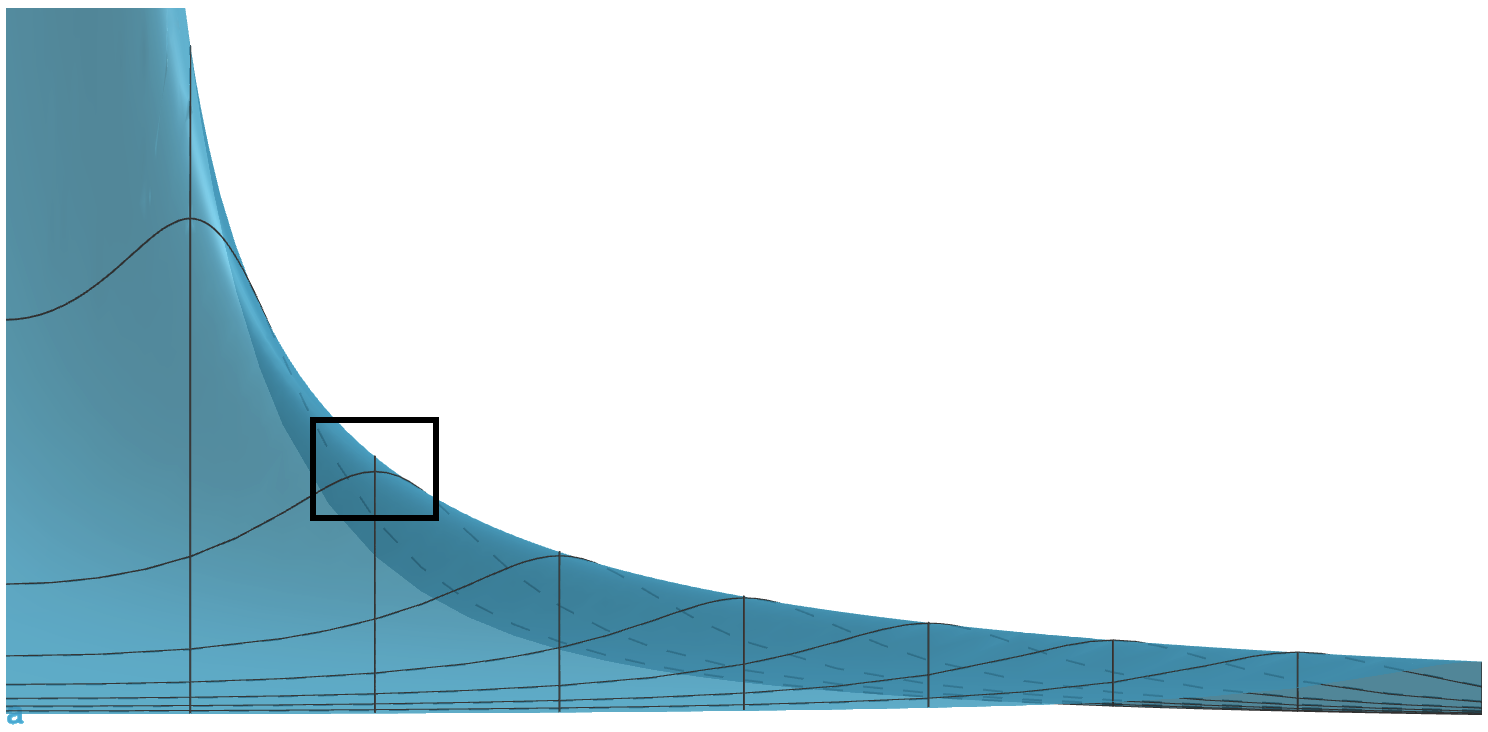
\includegraphics[width=0.9\linewidth]{../ExtFiles/resAmpb.png}
            \caption{Fixing $\omega_0$ vs. $\omega_1$.}
            \label{fig:resAmpb}
        \end{subfigure}
        \begin{subfigure}[b]{0.3\linewidth}
            \centering
            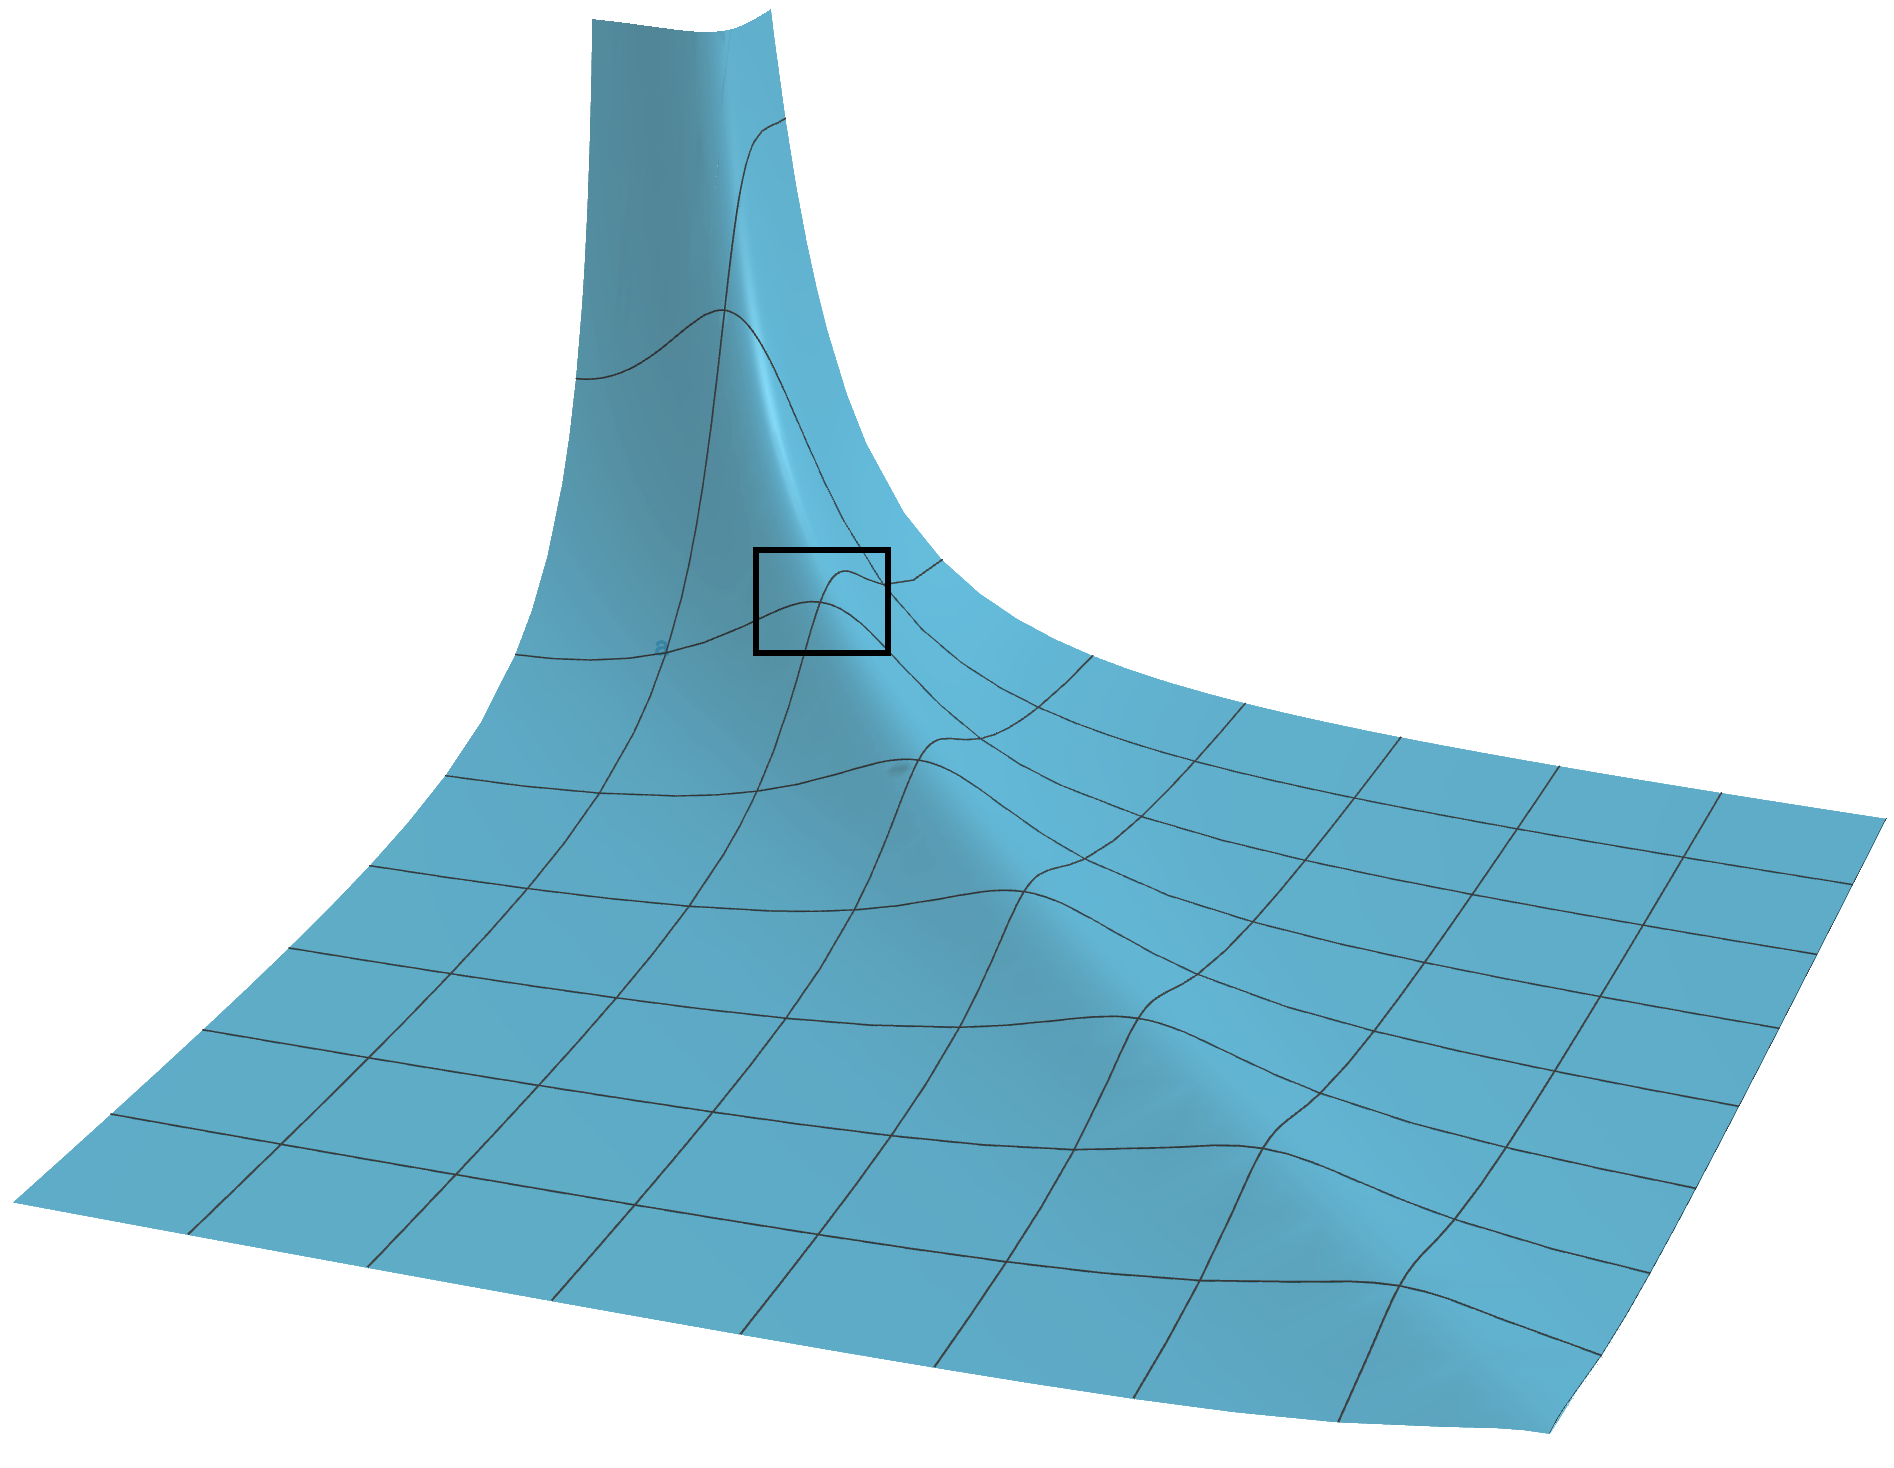
\includegraphics[width=0.9\linewidth]{../ExtFiles/resAmpc.png}
            \caption{$a_1(\omega_0,\omega_1)$.}
            \label{fig:resAmpc}
        \end{subfigure}\\[1em]
        \begin{subfigure}[b]{0.24\linewidth}
            \centering
            \begin{tikzpicture}
                \small
                \draw [stealth-stealth] (0,2.1) node[above]{$a_1$} -- (0,0) node[left]{${\color{white}\omega_1}$} -- (2.2,0) node[right]{${\color{grx}\omega_0}$ ${\color{orx}\omega_1}$};
    
                \draw [grx,thick] plot[domain=0:2,smooth] (\x,{1/((\x*\x-1)^2+1/4)^0.5});
                \draw [orx,thick] plot[domain=0:2,smooth] (\x,{1/((1-\x*\x)^2+\x*\x/4)^0.5});
            \end{tikzpicture}
            \caption{$\omega_1$ vs. $\omega_0$ profiles.}
            \label{fig:resAmpd}
        \end{subfigure}
        \caption{Oscillator resonance amplitude optimization.}
        \label{fig:resAmp}
    \end{figure}
    \begin{itemize}
        \item Note that for the entirety of what follows, we are in the underdamped case, so we \emph{always} have $\gamma<\omega_0$.
        \item Fix $\omega_1$. Varying $\omega_0$, we can see from Figure \ref{fig:resAmpa} that $a_1(\omega_0)$ is maximized when $\omega_0=\omega_1$.
        \begin{itemize}
            \item This \emph{resonance amplitude} is given by
            \begin{equation*}
                a_1(\omega_1,\omega_1) = \frac{F_1}{2m\gamma\omega_1}
                = \frac{F_1}{\lambda\omega_1}
            \end{equation*}
            \item Notice that the resonance amplitude grows as the damping $\lambda$ shrinks.
        \end{itemize}
        \item However, $a_1$ is a function of both $\omega_0$ \emph{and} $\omega_1$.
        \begin{itemize}
            \item Thus, it turns out that while $a_1(\omega_1,\omega_1)$ is a maximum when $\omega_1$ is fixed, it is \emph{not} a maximum when $\omega_0$ is fixed.
            \item This can be observed from the boxed area of Figure \ref{fig:resAmpb}; notice how the line going from left to right peaks where it crosses the line going into the page, but the line going into the page continues rising for a little bit before it peaks at the top of the blue manifold. Another perspective of the manifold is available in Figure \ref{fig:resAmpc}.
        \end{itemize}
        \item Indeed, $a_1$ reaches a \emph{true} maximum when we fix $\omega_0$ and shrink $\omega_1$ down to
        \begin{equation*}
            \omega_1 = \sqrt{\omega_0^2-2\gamma^2}
        \end{equation*}
        \begin{itemize}
            \item This can also be seen from Figures \ref{fig:resAmpb}-\ref{fig:resAmpc}. Notice how $\omega_1$ has to go a bit further into the page (i.e., has to \emph{shrink}) to reach the true maximum.
            \item We can also see this in Figure \ref{fig:resAmpd}, where it is observable that the orange line ($\omega_0$ fixed; $\omega_1$ varied) has a higher peak at a smaller value than the green line ($\omega_1$ fixed; $\omega_0$ varied).
            \item While the difference between $\omega_0$ and $\sqrt{\omega_0^2-2\gamma^2}$ is small (esp. for $\gamma$ small), it is still significant enough to merit a mention.
            \item Note that the \textbf{natural frequency} lies between $\omega_0$ and $\omega_1$ for such a maximum-amplitude driven-damped oscillator. Explicitly,
            \begin{equation*}
                \underbrace{\sqrt{\omega_0^2-0\gamma^2}}_{\omega_0} > \underbrace{\sqrt{\omega_0^2-\gamma^2}}_\omega
                > \underbrace{\sqrt{\omega_0^2-2\gamma^2}}_{\omega_1}
            \end{equation*}
            \item We have
            \begin{equation*}
                a_1(\omega_0,\sqrt{\omega_0^2-2\gamma^2}) = \frac{F_1}{2m\gamma\omega}
                = \frac{F_1}{\lambda\omega}
            \end{equation*}
            where $\omega$ is the natural frequency. Note that $a_1(\omega_0,\sqrt{\omega_0^2-2\gamma^2})>a_1(\omega_1,\omega_1)$ from above even though $\omega_1<\omega$ because $\omega_1$ was defined differently at the top.
        \end{itemize}
    \end{itemize}
    \item \textbf{Natural frequency} (of a harmonic oscillator): The frequency at which the oscillator oscillates when it is not being driven. \emph{Denoted by} $\bm{\omega}$. \emph{Given by}
    \begin{equation*}
        \omega = \sqrt{\omega_0^2-\gamma^2}
    \end{equation*}
    \begin{itemize}
        \item For an underdamped, driven oscillator, this is the frequency at which the transient term oscillates.
    \end{itemize}
    \item The amplitude and phase of the induced oscillation more generally.
    \begin{figure}[h!]
        \centering
        \begin{subfigure}[b]{0.4\linewidth}
            \centering
            \begin{tikzpicture}[scale=2]
                \small
                \draw [stealth-stealth] (0,2.1) node[above]{$a_1$} -- (0,0) -- (2.2,0) node[right]{$\omega_1$};
    
                \footnotesize
                \draw [dashed] (0.935,0) node[below]{$\sqrt{\omega_0^2-2\gamma^2}$} -- (0.935,2.066);
                \draw [<->,shorten <=1pt,shorten >=1pt] (0.935,1.461) -- node[below]{$\gamma$} (1.166,1.461);
                \node [left] at (0,1) {$\dfrac{F_1}{m\omega_0^2}$};
                \node [above right] at (1.08,1.77) {large $Q$};
                \node [below] at (0.4675,1.02) {small $Q$};
                
                \draw [ory,thick] plot[domain=0:2,samples=100,smooth] (\x,{1/((1-\x*\x)^2+\x*\x)^0.5});
                \draw [orx,thick] plot[domain=0:2,samples=100,smooth] (\x,{1/((1-\x*\x)^2+\x*\x/4)^0.5});
            \end{tikzpicture}
            \caption{Amplitude.}
            \label{fig:resa}
        \end{subfigure}
        \begin{subfigure}[b]{0.4\linewidth}
            \centering
            \begin{tikzpicture}[scale=2]
                \small
                \draw [stealth-stealth] (0,2.1) node[above]{$\theta_1$} -- (0,0) -- node[white,below]{$\sqrt{\omega_0^2-2\gamma^2}$} (2.2,0) node[right]{$\omega_1$};
    
                \footnotesize
                \draw [dashed] (0,1.8) node[left]{$\pi$} -- (2.1,1.8);
                \draw [dashed] (0,0.9) node[left]{$\dfrac{\pi}{2}$} -- (1,0.9) -- (1,0) node[below]{$\omega_0$};
                \node [left] at (1.05,1.5) {large $Q$};
                \node [below right=3pt] at (1.33,1.5) {small $Q$};
                
                \draw [ory,thick] plot[domain=0:2,samples=100,smooth] (\x,{0.9*(1+atan(3*(\x-1))/90)});
                \draw [orx,thick] plot[domain=0:2,samples=100,smooth] (\x,{0.9*(1+atan(20*(\x-1))/90)});
            \end{tikzpicture}
            \caption{Phase.}
            \label{fig:resb}
        \end{subfigure}
        \caption{Oscillator resonance amplitude and phase.}
        \label{fig:res}
    \end{figure}
    \begin{itemize}
        \item We can define the \textbf{width} and \textbf{half-width} of the oscillation.
        \item The quality factor is relevant here again, as well.
        \begin{itemize}
            \item Quantitative measure of the sharpness of the resonance peak.
            \item $Q=\omega_0/2\gamma$ also equals the ratio of the amplitude at resonance $F_1/2m\gamma\omega_0$ to the amplitude at $\omega_1=0$ $F_1/m\omega_0^2$.
        \end{itemize}
        \item The driving force creates the largest possible amplitude when it pulls on the particle with maximum strength slightly after the particle has passed the halfway point.
        \item Small forces can set up large resonances; allusion to the Millennium Bridge.
        \item On the phase.
        \begin{itemize}
            \item If the force is slowly oscillating, $\omega_1$ is small and $\theta_1\approx 0$ so that the induced oscillations are in phase with the force.
            \item Vice versa for very fast oscillations. Note that in this case, $a_1$ is very small. Additionally, the oscillations roughly correspond to those of a free particle under the applied oscillatory force; indeed, the half-period offset means that as soon as the particle crosses 0, the force is drawing it back toward zero!
            \item Right in the middle for resonance, that is, $\theta_1=\pi/2$. In this case, the induced oscillations lag behind the force by a quarter period.
        \end{itemize}
        \item Last note: $\gamma$ and $\lambda$ are only important in the region near resonance.
    \end{itemize}
    \item \textbf{Width} (of a resonance): The range of frequencies over which $a_1$ is large.
    \item \textbf{Half-width} (of a resonance): The offset of $\omega_1$ from $\omega_0$ at which the amplitude is reduced to $1/\sqrt{2}$ of its peak value. \emph{Given by} $\gamma$.
    \begin{itemize}
        \item If you approximate $\omega\approx\omega_0\pm\gamma$, then we can calculate that
        \begin{equation*}
            \frac{a_1(\omega_0,\omega_0\pm\gamma)}{a_1(\omega_0,\sqrt{\omega_0^2-2\gamma^2})} = \frac{\frac{F_1/m}{\sqrt{(\omega_0^2-(\omega_0+\gamma)^2)^2+4\gamma^2(\omega_0+\gamma)^2}}}{\frac{F_1/m}{\sqrt{\left( \omega_0^2-\sqrt{\omega_0^2-2\gamma^2}^2 \right)^2+4\gamma^2\sqrt{\omega_0^2-2\gamma^2}^2}}}
            % = \frac{\sqrt{4\gamma^4+4\gamma^2(\omega_0^2-2\gamma^2)}}{\sqrt{(-2\gamma\omega_0-\gamma^2)^2+4\gamma^2(\omega_0^2+2\gamma\omega_0+\gamma^2)}}
            = \frac{1}{\sqrt{2}}
        \end{equation*}
        \item Additionally, note that $\omega_1=\omega_0\pm\gamma$ makes the two terms in the denominator of $a_1$ equal each other.
    \end{itemize}
\end{itemize}


\subsection*{Section 2.7: General Periodic Force}
\begin{itemize}
    \item \marginnote{10/10:}Skipped in class.
\end{itemize}


\subsection*{Section 2.8: Impulsive Forces; The Green's Function Method}
\begin{itemize}
    \item Herein, we derive a method to obtain a solution to the damped driven harmonic oscillator equation
    \begin{equation*}
        m\ddot{x}+\lambda\dot{x}+kx = F(t)
    \end{equation*}
    for an arbitrary force function $F(t)$.
    \begin{itemize}
        \item Essentially, we will treat $F(t)$ as if it is impacting on the oscillator as an infinite sum of infinitesimally small \textbf{impulses}.
        \item This is where we're going.
    \end{itemize}
    \item \textbf{Impulse}: The change in momentum of a particle during the time at which a large force momentarily acts on it. \emph{Denoted by} $\bm{I}$. \emph{Given by}
    \begin{equation*}
        I = \Delta p
        = p(t+\Delta t)-p(t)
        = \int_t^{t+\Delta t}F\dd{t}
    \end{equation*}
    \item A good approximation of a collision: Let the momentum of the particle change discontinuously under an impulse $I$ delivered "instaneously," that is, with $F\to\infty$ and $\Delta t\to 0$.
    \begin{itemize}
        \item Of course, this is not physically accurate, but it is a good approximation.
    \end{itemize}
    \item The effect of an impulse $I$ delivered at time $t=0$ to an underdamped harmonic oscillator at rest at the equilibrium position.
    \begin{itemize}
        \item The trajectory for this situation is
        \begin{equation*}
            x(t) =
            \begin{cases}
                0 & t<0\\
                \frac{v_0}{\omega}\e[-\gamma t]\sin(\omega t) & t>0
            \end{cases}
        \end{equation*}
        \begin{itemize}
            \item We can learn that $a=v_0/\omega$ by taking the derivative of the general solution and solving for $\dot{x}(0)$.
            \item We use $\sin$ instead of $\cos$ to encapsulate the phase shift that has us starting at the origin at $t=0$. $\sin$ is the only phase shift that keeps $x(t)$ continuous.
        \end{itemize}
        \item Calculate the velocity $v_0$ of the oscillator after the impulse.
        \begin{itemize}
            \item We have that
            \begin{equation*}
                I = \Delta p = p-0 = p = mv_0
            \end{equation*}
            so that
            \begin{equation*}
                v_0 = \frac{I}{m}
            \end{equation*}
        \end{itemize}
        \item Thus, the complete trajectory is
        \begin{equation*}
            x(t) =
            \begin{cases}
                0 & t<0\\
                \frac{I}{m\omega}\e[-\gamma t]\sin(\omega t) & t>0
            \end{cases}
        \end{equation*}
        \item It will look like Figure \ref{fig:dampedOscillatorb} but phase shifted right by $\pi/2$.
    \end{itemize}
    \item What if while the oscillator is recovering from a blow, it receives another one?
    \begin{itemize}
        \item Suppose this second impulse $I_2$ occurs at time $t_2$.
        \item Naturally, the oscillator will have some velocity $v_1$ at time $t_2$ due to the initial impulse $I_1$. Likewise, its momentum will be $p_1=mv_1$.
        \item Impulse $I_2$ changes $p_1$ to $p_1+\Delta p=p_1+I_2$. In particular, it changes the velocity from $v_1$ to $v_2=v_1+\Delta v$ where $I_2=m\Delta v$.
        \item Thus, a second impulse essentially resets the velocity to yet another value, from which point we continue decaying oscillation with this new "initial" velocity. However, mathematically, this is equivalent to superimposing the motion of the particle from rest at equilibrium subject to $I_2$ on top of the existing result of subjection to $I_1$ at $t=0$. This is key.
    \end{itemize}
    \item Generalizing to the case where the oscillator is subjected to a series of blows $I_1,\dots,I_n$.
    \begin{itemize}
        \item Invoking the superposition principle mentioned above, we have
        \begin{equation*}
            x(t) = \sum_rG(t-t_r)I_r+\text{transient}
        \end{equation*}
        where
        \begin{equation*}
            G(t-t_r) =
            \begin{cases}
                0 & t<t_r\\
                \frac{1}{m\omega}\e[-\gamma(t-t_r)]\sin\omega(t-t_r) & t>t_r
            \end{cases}
        \end{equation*}
        for all $r=1,\dots,n$.
    \end{itemize}
    \item Recall that the 2-variable function $G(t,t_r)=G(t-t_r)$ described above is the \textbf{Green's function} of the oscillator.
    \begin{itemize}
        \item Meaning: Represents the response to a blow of unit impulse at time $t_r$.
    \end{itemize}
    \item Solving the original equation.
    \begin{itemize}
        \item Partition $F(t)$ into intervals of impulses $F(t)\Delta t$.
        \item Taking the limit as $\Delta t\to 0$ and summing as above, we arrive at
        \begin{equation*}
            x(t) = \int_{t_0}^tG(t-t')F(t')\dd{t'}+\text{transient}
        \end{equation*}
    \end{itemize}
    \item \textcite{bib:KibbleBerkshire} goes through an example.
\end{itemize}


\subsection*{Section 2.9: Collision Problems}
\begin{itemize}
    \item Skipped in class.
\end{itemize}


\subsection*{Section 2.10: Summary}
\begin{itemize}
    \item Some good ideas.
    \item Note: Resonance can occur in any system subjected to periodic forces, including ones that are not harmonic!
    \begin{itemize}
        \item The true characteristic of resonance is when the forcing frequency is approximately the natural frequency.
    \end{itemize}
\end{itemize}




\end{document}